\chapter{Đại cương về tập hợp}

\section{Tập hợp}

\subsection*{Mở đầu về tập hợp}

Một tập hợp (set) bao gồm các phần tử khác nhau. Để biểu diễn tập hợp
ta có hai cách.

\begin{enumerate}
    \item Liệt kê. Ví dụ $A = \{ 1, 2, 3, 4 \}$, $B = \{ a, b , c \}$
    \item Sử dụng tính chất đặc trưng. Ví dụ $A = \{ a \in \NN^* : a < 5 \}$.
\end{enumerate}

Ở đây hai cách biểu diễn tập hợp $A$ là giống nhau.

\begin{definition}[Tập hợp rỗng]
    Tập hợp rỗng không chứa phần tử nào, ký hiệu là $\emptyset$.
\end{definition}

\begin{definition}[Tập hợp con]
    Xét tập hợp $A$. Tập hợp $B$ được gọi là \textbf{tập hợp con} của tập $A$
    nếu mọi phần tử của $B$ đều nằm trong $A$. Nói cách khác với mọi $b \in B$ thì
    $b \in A$. Ta ký hiệu $B \subset A$.
\end{definition}

\begin{remark}
    Tập hợp rỗng là con của mọi tập hợp.
\end{remark}

Dễ thấy rằng mọi tập hợp là tập hợp con của chính nó. Do đó tập con này được gọi là
tập con tầm thường (trivial subset). Để ký hiệu một tập con có thể bằng tập chứa nó
ta viết $B \subseteq A$. Trong trường hợp $B$ là tập con của $A$ nhưng không bằng 
$A$ ta có thể viết $B \subsetneq A$.

\subsection*{Toán tử trên tập hợp}

Chúng ta xem xét 3 toán tử cơ bản trên tập hợp là \textit{giao}, \textit{hợp}
và \textit{hiệu} của hai tập hợp. Để biểu diễn các toán tử này ta có thể dùng 
biểu đồ Venn.

\begin{definition}[Giao của hai tập hợp]
    Giao của hai tập hợp $A$ và $B$ là tập hợp các phần tử thuộc cả $A$ và $B$.
    \begin{equation}
        A \cap B = \{ x : x \in A \text{ và } x \in B \}
    \end{equation}
\end{definition}

\begin{figure}[htb]
    \centering
    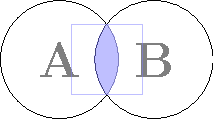
\includegraphics[page=1]{figures/set/venn_diagram.pdf}
    \caption{Phép giao hai tập hợp}
    \label{set1}
\end{figure}

Hình \ref{set1} là biểu đồ Venn tương ứng của phép giao hai tập hợp. Khi giao của hai 
tập hợp $A$ và $B$ là rỗng thì ta nói hai tập rời nhau. Ký hiệu $A \cap B = \emptyset$.

\begin{definition}[Hợp của hai tập hợp]
    Hợp của hai tập hợp $A$ và $B$ là tập hợp các phần tử thuộc $A$ hoặc $B$.
    \begin{equation}
        A \cup B = \{ x : x \in A \text{ hoặc } x \in B \}
    \end{equation}
\end{definition}

Hình \ref{set2} là biểu đồ Venn tương ứng của phép hợp hai tập hợp.

\begin{figure}[htb]
    \centering
    \includegraphics[page=2]{figures/set/venn_diagram.pdf}
    \caption{Phép hợp hai tập hợp}
    \label{set2}
\end{figure}

\begin{definition}[Hiệu của hai tập hợp]
    Hợp của hai tập hợp $A$ và $B$ là tập hợp các phần tử thuộc $A$ nhưng không thuộc $B$.
    \begin{equation}
        A \backslash B = \{ x : x \in A \text{ và } x \not\in B \}
    \end{equation}
\end{definition}

Hình \ref{set3} là biểu đồ Venn tương ứng của hiệu hai tập hợp.

\begin{figure}[ht]
    \centering
    \includegraphics[page=3]{figures/set/venn_diagram.pdf}
    \caption{Phép hiệu hai tập hợp}
    \label{set3}
\end{figure}

\subsection*{Lực lượng của tập hợp}

Để chỉ số lượng phần tử của một tập hợp ta dùng khái niệm lực lượng của tập hợp.

Ký hiệu lực lượng của tập hợp $A$ là $\lvert A \rvert$.

Khi một tập hợp có vô số phần tử, ta gọi đó là tập vô hạn. Ngược lại ta gọi là
tập hữu hạn.

\begin{example}
    Các tập hợp số thông dụng $\NN$, $\ZZ$, $\QQ$, $\RR$ là các tập vô hạn.

    Tập hợp $A = \{ 1, 2, 3, 4, 5 \}$ là tập hữu hạn có 5 phần tử. Ký hiệu
    $\lvert A \rvert = 5$.
\end{example}

Từ biểu đồ Venn chúng ta cũng có thể tìm được công thức tính lực lượng của tập
$A \cup B$.

\begin{figure}[ht]
    \centering
    \includegraphics[page=4]{figures/set/venn_diagram.pdf}
    \caption{Nguyên lý bù trừ cho hai tập hợp}
    \label{set4}
\end{figure}

Dựa vào hình ta có thể suy ra công thức sau

\begin{equation}
    \lvert A \cup B \rvert = \lvert A \rvert + \lvert B \rvert - \lvert A \cap B \rvert
\end{equation}

\section{Ánh xạ}

\subsection*{Ánh xạ}

Cho 2 tập hợp $X$ và $Y$. Ánh xạ $f$ biến một phần tử $x \in X$ thành một và chỉ một phần tử $y \in Y$.

Ta ký hiệu
\[f: X \to Y, \; f(x) = y\]

Khi đó, $X$ được gọi là tập nguồn (domain) và $Y$ là tập đích (image).

Ánh xạ có 3 loại:

\begin{itemize}
    \item \textbf{Đơn ánh} (hay \textbf{injection}): Hai phần tử khác nhau của tập nguồn cho hai ảnh khác nhau. Tức là với mọi $x_1, x_2 \in X$ mà $x_1 \neq x_2$, thì $f(x_1) \neq f(x_2)$
    \item \textbf{Toàn ánh} (hay \textbf{Surjection}): Mọi phần tử $y \in Y$ đều có ít nhất một phần tử $x \in X$ mà $f(x) = y$. Nói cách khác với mỗi phần tử trong $Y$ ta đều tìm được phần tử thuộc $X$ biến thành nó
    \item \textbf{Song ánh} (hay \textbf{Bijection}): Nếu ánh xạ đó vừa là đơn ánh, vừa là toàn ánh
\end{itemize}

Dựa vào định nghĩa và hình vẽ, ta có thể rút ra kết luận như sau
\begin{itemize}
    \item Đối với đơn ánh, do mọi phần tử của $X$ đều có ảnh ở $Y$, tuy nhiên có thể có phần tử ở $Y$ không do phần tử nào của $X$ biến thành (trong hình là 5). Do đó $\lvert X \rvert \leqslant \lvert Y \rvert$.
    \item Đối với toàn ánh, mọi phần tử của $Y$ đều có nguồn gốc xuất xứ, tuy nhiên có thể có phần tử của $X$ không biến thành $y$ nào của $Y$ (trong hình là $e$). Do đó $\lvert X \rvert \geqslant \lvert Y \rvert$.
    \item Đối với song ánh, do là kết hợp giữa đơn ánh và toàn ánh, khi đó dấu đẳng thức xảy ra, $\lvert X \rvert = \lvert Y \rvert$.
\end{itemize}

\begin{figure}[htb]
    \centering
    \begin{subfigure}{0.4\textwidth}
        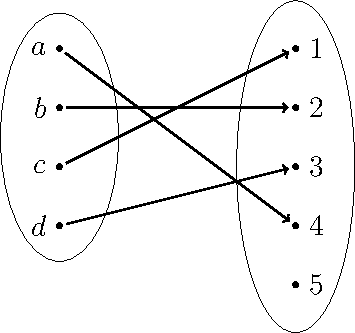
\includegraphics[page=1]{figures/maps.pdf}
        \caption{Đơn ánh}
    \end{subfigure}
    \hfill
    \begin{subfigure}{0.4\textwidth}
        \includegraphics[page=2]{figures/maps.pdf}
        \caption{Toàn ánh}
    \end{subfigure}
    \hfill
    \begin{subfigure}{0.4\textwidth}
        \includegraphics[page=3]{figures/maps.pdf}
        \caption{Song ánh}
    \end{subfigure}
    \caption{Các loại ánh xạ}
\end{figure}

\subsection*{Hàm số}

Khi 2 tập nguồn và đích của ánh xạ là 2 tập hợp số, ta có hàm số.

\begin{example}
    Hàm số $f: \RR \rightarrow \RR$ với $y = f(x) = x^3 + x + 1$. Ở đây $X \equiv \RR$ và $Y \equiv \RR$.
\end{example}

Lưu ý rằng tập nguồn và đích không nhất thiết là tập hợp số cơ bản ($\QQ, \RR$) mà cũng có thể là tích Descartes của chúng.

\begin{example}
    Hàm số $f: \RR \times \RR \rightarrow \RR$ với $z = f(x, y) = x + y + xy$. Ở đây $X \equiv \RR$, $Y \equiv \RR$ và $Z \equiv \RR$.
\end{example}

Chúng ta còn một cách gọi khác cho đơn ánh, toàn ánh, song ánh trong tiếng Anh.

\begin{table}[ht]
    \centering
    \begin{tabular}{| l | l | l |}
        \hline
        đơn ánh & injection & one-to-one map \\
        \hline
        toàn ánh & surjection & onto map \\
        \hline
        song ánh & bijection & one-to-one and onto map \\
        \hline
    \end{tabular}

    \caption{Thuật ngữ tiếng Anh cho ánh xạ}
\end{table}

\begin{example}
    Hàm số $f: \RR \rightarrow \RR$ cho bởi $y = f(x) = x^3$ là song ánh.

    \begin{proof}
        Ta thấy nếu $f(x_1) = f(x_2)$, tương đương $x_1^3 = x_2^3$ nên $x_1 = x_2$. Do đó $f$ là đơn ánh.

        Với mọi $y = x^3 \in \RR$, do căn bậc 3 luôn tồn tại nên ta có $x = \sqrt[3]{y}$. Nghĩa là luôn tồn tại $x$ để $f(x) = y$ với mọi $y \in \RR$. Do đó $f$ là toàn ánh.

        Kết luận $f$ là song ánh.
    \end{proof}
\end{example}

\subsection*{Đồng biến và nghịch biến}

\begin{definition}
    Xét hàm số $f(x)$ xác định trên khoảng $(a, b)$. Ta nói $f(x)$ \textbf{đồng biến} (tăng) trên $(a, b)$ nếu với mọi $x_1, x_2 \in (a, b)$ mà $x_1 < x_2$ ta có $f(x_1) < f(x_2)$.
\end{definition}

Tương tự $f(x)$ \textbf{nghịch biến} (giảm) trên $(a, b)$ nếu với mọi $x_1, x_2 \in (a, b)$ mà $x_1 < x_2$ ta có $f(x_1) > f(x_2)$.

Lưu ý ở các so sánh trên dấu bằng có thể xảy ra. Khi đó hàm số được gọi là tăng \textit{không nghiêm ngặt} (hoặc giảm \textit{không nghiêm ngặt}).

Nếu hàm số đồng biến (hoặc nghịch biến) trên khoảng xác định nào đó thì ta nói hàm số đơn điệu trên khoảng đó.

Đồ thị của hàm số khi đồng biến sẽ đi lên (theo chiều từ trái sang phải), và đi xuống nếu nghịch biến.

\begin{example}
    Khảo sát sự biến thiên của hàm số $f(x) = x^2 + 3$.

    Để khảo sát sự biến thiên, một cách làm đơn giản theo định nghĩa là ta xét $x_1 < x_2$ và so sánh $f(x_1)$ với $f(x_2)$.

    Ta có $f(x_1) - f(x_2) = x_1^2 + 3 - x_2^2 - 3 = (x_1 - x_2)(x_1 + x_2)$

    Do $x_1 < x_2$, nên với $x_1, x_2 > 0$ thì $x_1 + x_2 > 0$ và $x_1 - x_2 < 0$. Suy ra $f(x_1) - f(x_2) < 0$ và từ đó $f(x_1) < f(x_2)$. Như vậy $f(x)$ đồng biến trên $(0, +\infty)$.

    Tương tự, khi $x_1, x_2 < 0$ thì $x_1 + x_2 < 0$. Khi đó $f(x_1) > f(x_2)$ nên $f(x)$ nghịch biến trên $(-\infty, 0)$.
\end{example}

Để thể hiện sự biến thiên của hàm số ta sử dụng bảng biến thiên.

Đối với hàm số $y = x^2 + 3$ ở trên bảng biến thiên có dạng:

\begin{figure}[bh]
    \centering
    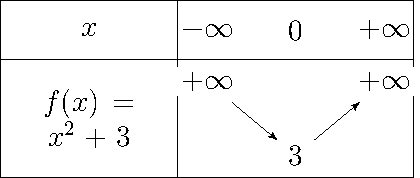
\includegraphics[page=1]{figures/table_of_variation.pdf}
    \caption{Bảng biến thiên hàm số $y=x^2 + 3$}
\end{figure}

Ta đã chứng minh được hàm số nghịch biến trên $(-\infty, 0)$ và đồng biến trên $(0, +\infty)$, giá trị $f(0) = 3$ nên bảng biến thiên thể hiện sự tăng giảm trên các khoảng. Dựa vào bảng biến thiên ta có thể hình dung ra dạng của đồ thị hàm số.

\subsection*{Đồ thị hàm số}

Để biểu diễn sự phụ thuộc của biến $y$ theo biến $x$, hay nói cách khác là biểu diễn hàm số $y=f(x)$ ta có thể dùng đồ thị.

Đồ thị được vẽ trên hệ tọa độ Descartes $Oxy$. Bảng biến thiên cho ta thấy tính đơn điệu trên các khoảng xác định, và đồ thị sẽ cho ta thấy rõ hơn độ "cong" của những đường cong.

\begin{example}
    Với hàm số $y = x^2 + 3$ ở trên. Đồ thị hàm số có dạng như hình \ref{func1}.

    Với hàm số $y = \dfrac{1}{x}$. Ta thấy rằng hàm số không xác định tại $x=0$. Khảo sát sự biến thiên như bên trên ta thấy hàm số nghịch biến ở hai khoảng xác định là $(-\infty, 0)$ và $(0, +\infty)$. Đồ thị hàm số có dạng như hình \ref{func2}.
\end{example}

\begin{figure}
    \centering
    \begin{subfigure}{0.4\textwidth}
        \includegraphics[page=2]{figures/table_of_variation.pdf}
        \caption{Đồ thị hàm số $y=x^2 + 3$}
        \label{func1}
    \end{subfigure}
    \hfill
    \begin{subfigure}{0.55\textwidth}
        \includegraphics[page=3]{figures/table_of_variation.pdf}
        \caption{Đồ thị hàm số $y = \dfrac{1}{x}$}
        \label{func2}
    \end{subfigure}
    \caption{Đồ thị một số hàm thông dụng}
\end{figure}
Từ đồ thị của 2 hàm số trên ta thấy rằng mặc dù cùng là nghịch biến trên $(-\infty, 0)$ nhưng nghịch biến của $y=x^2+3$ nhìn "nhẹ nhàng" hơn. Trong khi  đồ thị $y = \dfrac{1}{x}$ thì ban đầu "nhẹ nhàng", sau thì như "rơi tự do".

\section{Một số loại hàm số}

Một số hàm số có tính chất đặc biệt giúp chúng ta tiết kiệm công sức trong chứng minh, tính toán.

\subsection*{Hàm chẵn và hàm lẻ}

Xét hàm số $y=f(x)$ xác định trên miền $D$ có tính đối xứng, nghĩa là với mỗi phần tử dương $x \in D$ thì có phần tử âm $-x \in D$ hoặc ngược lại. Khi đó

\begin{definition}[Hàm số chẵn]
    Hàm số $y=f(x)$ được gọi là \textbf{hàm số chẵn} nếu với mọi $x \in D$ ta có $f(-x) = f(x)$.
\end{definition}

Ví dụ như hàm số $y = x^2 + 3$ ở trên là một hàm chẵn vì với mọi $x \in \RR$, $f(x) = x^2 + 3 = (-x)^2 + 3 = f(-x)$. Dễ thấy rằng hàm chẵn đối xứng qua trục tung. Dựa vào tính chất này, trong lúc khảo sát hoặc tính toán đôi khi ta chỉ cần quan tâm một bên trục tung, bên kia tương tự.

\begin{definition}[Hàm số lẻ]
    Hàm số $y=f(x)$ được gọi là \textbf{hàm số lẻ} nếu với mọi $x \in D$ ta có $f(-x) = -f(x)$.
\end{definition}

Ví dụ như hàm số $y = \dfrac{1}{x}$ ở trên là một hàm lẻ vì với mọi $x \in (-\infty, 0) \cup (0, +\infty)$, $f(-x) = \dfrac{1}{-x} = -\dfrac{1}{x} = -f(x)$. Dễ thấy rằng hàm lẻ đối xứng qua gốc tọa độ $O$.

\subsection*{Hàm cộng tính}

Xét hàm số $y=f(x)$ xác định trên miền $D$. 

\begin{definition}[Hàm cộng tính]
    Hàm số $y = f(x)$ được gọi là \textbf{cộng tính} nếu với mọi $x, y \in D$ ta có $f(x+y) = f(x) + f(y)$.
\end{definition}

\begin{example}
    Hàm số $y = 2x$ trên $\RR$ là hàm cộng tính vì với mọi $x, y \in \RR$, ta có $f(x+y) = 2(x+y) = 2x + 2y = f(x) + f(y)$.
\end{example}

\subsection*{Hàm nhân tính}

Tương tự hàm cộng tính, ta định nghĩa hàm nhân tính.

\begin{definition}[Hàm nhân tính]
    Hàm số $y = f(x)$ được gọi là \textbf{nhân tính} nếu với mọi $x, y \in D$
    ta có $f(xy) = f(x) \cdot f(y)$.
\end{definition}

Hàm nhân tính quan trọng được sử dụng trong số học là hàm $\varphi$ Euler về số lượng các số nguyên tố cùng nhau với số nguyên dương $n$. Nếu một hàm số học là nhân tính thì chúng ta chỉ cần quan tâm giá trị của hàm số đó tại các số nguyên tố là đủ.

\subsection*{Hàm tuần hoàn}

Xét hàm số $y=f(x)$ xác định trên miền $D$.

\begin{definition}[Hàm tuần hoàn]
    Hàm số $y=f(x)$ được gọi là \textbf{tuần hoàn} nếu tồn tại số $T$ sao cho $f(x+T) = f(x)$ với mọi $x \in D$.
\end{definition}

Nói cách khác, hàm số sẽ lặp lại sau một đoạn nhất định.

Số $T$ nhỏ nhất thỏa mãn $f(x+T) = f(x)$ được gọi là \textbf{chu kỳ} của hàm tuần hoàn. Vì sao lại là nhỏ nhất?

Ta thấy rằng, nếu $f(x+T) = f(x)$ với mọi $x \in D$, ta thay $x$ bởi $x + T$ thì thu được $f(x + T + T) = f(x+T)$, hay $f(x+2T) = f(x+T)$. Suy ra $f(x+2T) = f(x+T) = f(x)$. Như vậy thì sau $2T$ hàm số cũng lặp lại đúng trạng thái đó. Tương tự cho $3T$, $4T$, .... Nên số $T$ nhỏ nhất thỏa mãn đẳng thức $f(x+T) = f(x)$ sẽ là chu kỳ.

\begin{example}
    Hàm số $y = \sin(x)$ là hàm tuần hoàn với chu kỳ $T = 2\pi$. Do đó chúng ta chỉ cần khảo sát hàm số trong khoảng $(-\pi, \pi)$ thôi là đủ.
\end{example}

\section{Phép quy nạp toán học}

Giả sử ta muốn chứng minh một mệnh đề $P$ đúng với mọi $n \geqslant 1$. Phép quy nạp toán học hoạt động theo ba bước như sau

\begin{enumerate}
	\item Chứng minh mệnh đề $P$ đúng với $n=1$ (bước cơ sở)
	\item Giả sử mệnh đề $P$ đúng với $n = k \geqslant 1$. Đây gọi là giả thiết quy nạp
	\item Chứng minh mệnh đề $P$ đúng với $n = k+1$ từ giả thiết quy nạp bên trên
\end{enumerate}

Như vậy phép quy nạp toán học hoạt động theo bậc thang. Từ giả thiết quy nạp mệnh đề $P$ đúng với $n = 1$, theo chứng minh ở bước (3) thì nó cũng đúng ở bước $n = 1+1 = 2$. Do $P$ đúng với $n=2$ nên cũng đúng ở $n=3$. Cứ tiếp tục như vậy $P$ sẽ đúng với mọi $n \geqslant 1$. Đây là sự hiệu quả đáng kinh ngạc của phép quy nạp toán học.

\begin{example}
	Chứng minh công thức tổng quát cho tổng $1 + 2 + \ldots + n$ là $\dfrac{n(n+1)}{2}$.
	
	Với $n = 1$ thì $1 = \dfrac{1 (1 + 1)}{2}$. Như vậy công thức đúng cho $n = 1$. Đây là bước cơ sở.
	
	Giả sử mệnh đề đúng với $n = k \geqslant 1$. Nghĩa là $1 + 2 + \ldots + k = \dfrac{k(k+1)}{2}$. Đây là giả thiết quy nạp.
	
	Bây giờ ta cần chứng minh mệnh đề đúng với $n = k+1$. Nghĩa là cần chứng minh $1 + 2 + \ldots + k + (k+1) = \dfrac{(k+1)(k+2)}{2}$.
	
	Từ giả thiết quy nạp ta suy ra
	\begin{align*}
		1 + 2 + \ldots + k + (k+1) = & \dfrac{k(k+1)}{2} + (k+1) \\ = & \dfrac{k(k+1) + 2(k+1)}{2} \\ = & \dfrac{(k+1)(k+2)}{2}
	\end{align*}
	
	Vậy là ta đã có điều cần chứng minh, và công thức đã được chứng minh đúng với mọi $n \geqslant 1$.
\end{example}

\begin{remark}
	Tùy thuộc bài toán, bước cơ sở có thể không phải $1$ mà là một số nguyên dương nào đó khác.
\end{remark}